%%
%% This is file `tikzposter-template.tex',
%% generated with the docstrip utility.
%%
%% The original source files were:
%%
%% tikzposter.dtx  (with options: `tikzposter-template.tex')
%%
%% This is a generated file.
%%
%% Copyright (C) 2014 by Pascal Richter, Elena Botoeva, Richard Barnard, and Dirk Surmann
%%
%% This file may be distributed and/or modified under the
%% conditions of the LaTeX Project Public License, either
%% version 2.0 of this license or (at your option) any later
%% version. The latest version of this license is in:
%%
%% http://www.latex-project.org/lppl.txt
%%
%% and version 2.0 or later is part of all distributions of
%% LaTeX version 2013/12/01 or later.
%%


\documentclass{tikzposter} %Options for format can be included here

\usepackage{todonotes}

\usepackage[tikz]{bclogo}
\usepackage{lipsum}
\usepackage{amsmath}

\usepackage{booktabs}
\usepackage{longtable}
\usepackage[absolute]{textpos}
\usepackage[it]{subfigure}
\usepackage{graphicx}
\usepackage{cmbright}
%\usepackage[default]{cantarell}
%\usepackage{avant}
%\usepackage[math]{iwona}
\usepackage[math]{kurier}
\usepackage[T1]{fontenc}


%% add your packages here
\usepackage{hyperref}
% for random text
\usepackage{lipsum}
\usepackage[english]{babel}
\usepackage[pangram]{blindtext}

\colorlet{backgroundcolor}{blue!10}

 % Title, Author, Institute
\title{Disaster Tweets Prediction Using BERT}
\author{Ran Liu}
\institute{Institute of Information Engineering, \\ \bigskip
Chinese Academy of Sciences, China
}
%\titlegraphic{logos/tulip-logo.eps}

%Choose Layout
\usetheme{Wave}

%\definebackgroundstyle{samplebackgroundstyle}{
%\draw[inner sep=0pt, line width=0pt, color=red, fill=backgroundcolor!30!black]
%(bottomleft) rectangle (topright);
%}
%
%\colorlet{backgroundcolor}{blue!10}

\begin{document}


\colorlet{blocktitlebgcolor}{blue!23}

 % Title block with title, author, logo, etc.
\maketitle

\begin{columns}
 % FIRST column
\column{0.5}% Width set relative to text width

%%%%%%%%%% -------------------------------------------------------------------- %%%%%%%%%%
 %\block{Main Objectives}{
%  	      	\begin{enumerate}
%  	      	\item Formalise research problem by extending \emph{outlying aspects mining}
%  	      	\item Proposed \emph{GOAM} algorithm is to solve research problem
%  	      	\item Utilise pruning strategies to reduce time complexity
%  	      	\end{enumerate}
%%  	      \end{minipage}
%}
%%%%%%%%%% -------------------------------------------------------------------- %%%%%%%%%%


%%%%%%%%%% -------------------------------------------------------------------- %%%%%%%%%%
\block{Introduction}{
  Twitter has become an important communication channel in times of emergency. But it’s not always clear whether a person’s words are actually announcing a disaster. For instance, "\ \emph{Look at the sky last night it was ablaze!}\ " In this tweet, The author explicitly uses the word “\emph{ablaze}” which is related to disaster, but actually it is an exaggerated expression. Our goal is to resolve this problem. \bigskip
  \\
  Concretely, given a set of labeled data, we will use them to train a text classifier and use it to predict whether a tweet is about disaster or not. \bigskip
  \\
 In this paper, we first analyze the training set, including calculate distribution of characters and tokens of texts, then convert texts into standard input format which BERT can process. After that, we fine-tune BERT to adapt to disaster tweets prediction task. Our method has achieved good results, ranking top 2.3$\%$ in Kaggle competition.
}
%%%%%%%%%% -------------------------------------------------------------------- %%%%%%%%%%


%%%%%%%%%% -------------------------------------------------------------------- %%%%%%%%%%
\block{Related Work}{
\begin{itemize}
    \item
    \textbf{Rule-Based methods} classify texts into different categories using a set of pre-defined rules. The kind of methods are easy to implement and fast when running, also have good interpretability, while require a lot of manpower and time. What's worse, when facing a new problem, previous rules may become useless.
    

    \item
    \textbf{Statistical methods}, such as Naïve Bayes, support vector machines, hidden Markov model, and random forests, are more accurate than rule-based methods. On the other hand, statistical methods cannot take full advantage of large training data because the features are pre-defined.

    \item
    \textbf{Deep learning} which is represented by Convolutional Neural Network and Long Short-Term Memory Network, is the current mainstream method. It has strong ability to capture deep contexual features and can improve performance obviously. But weak interpretability and extreme reliance on large amount of training data are its main drawbacks.
\end{itemize}


}
%%%%%%%%%% -------------------------------------------------------------------- %%%%%%%%%%


%%%%%%%%%% -------------------------------------------------------------------- %%%%%%%%%%

%\note{Note with default behavior}

%\note[targetoffsetx=12cm, targetoffsety=-1cm, angle=20, rotate=25]
%{Note \\ offset and rotated}

 % First column - second block


%%%%%%%%%% -------------------------------------------------------------------- %%%%%%%%%%
\block{Dataset}{
  	The training set has a total of 7631 tweets, consisting of 3721 tweets about disaster and 3892 tweets which are not about disaster. \\ \\
    The maximum character length of text in training set is 157 and minimun is 7, with an average of 101 characters. \\ \\
    Since BERT takes token as word vector unit, we also calculate token statistics of training set. The maximum token length of text is 84 and minimun is 3, with an average of 33 tokens. \\ \\
    Distribution of character and token length are as follows.

    \begin{minipage}{0.5\linewidth}
      \centering
      \begin{tikzfigure}
        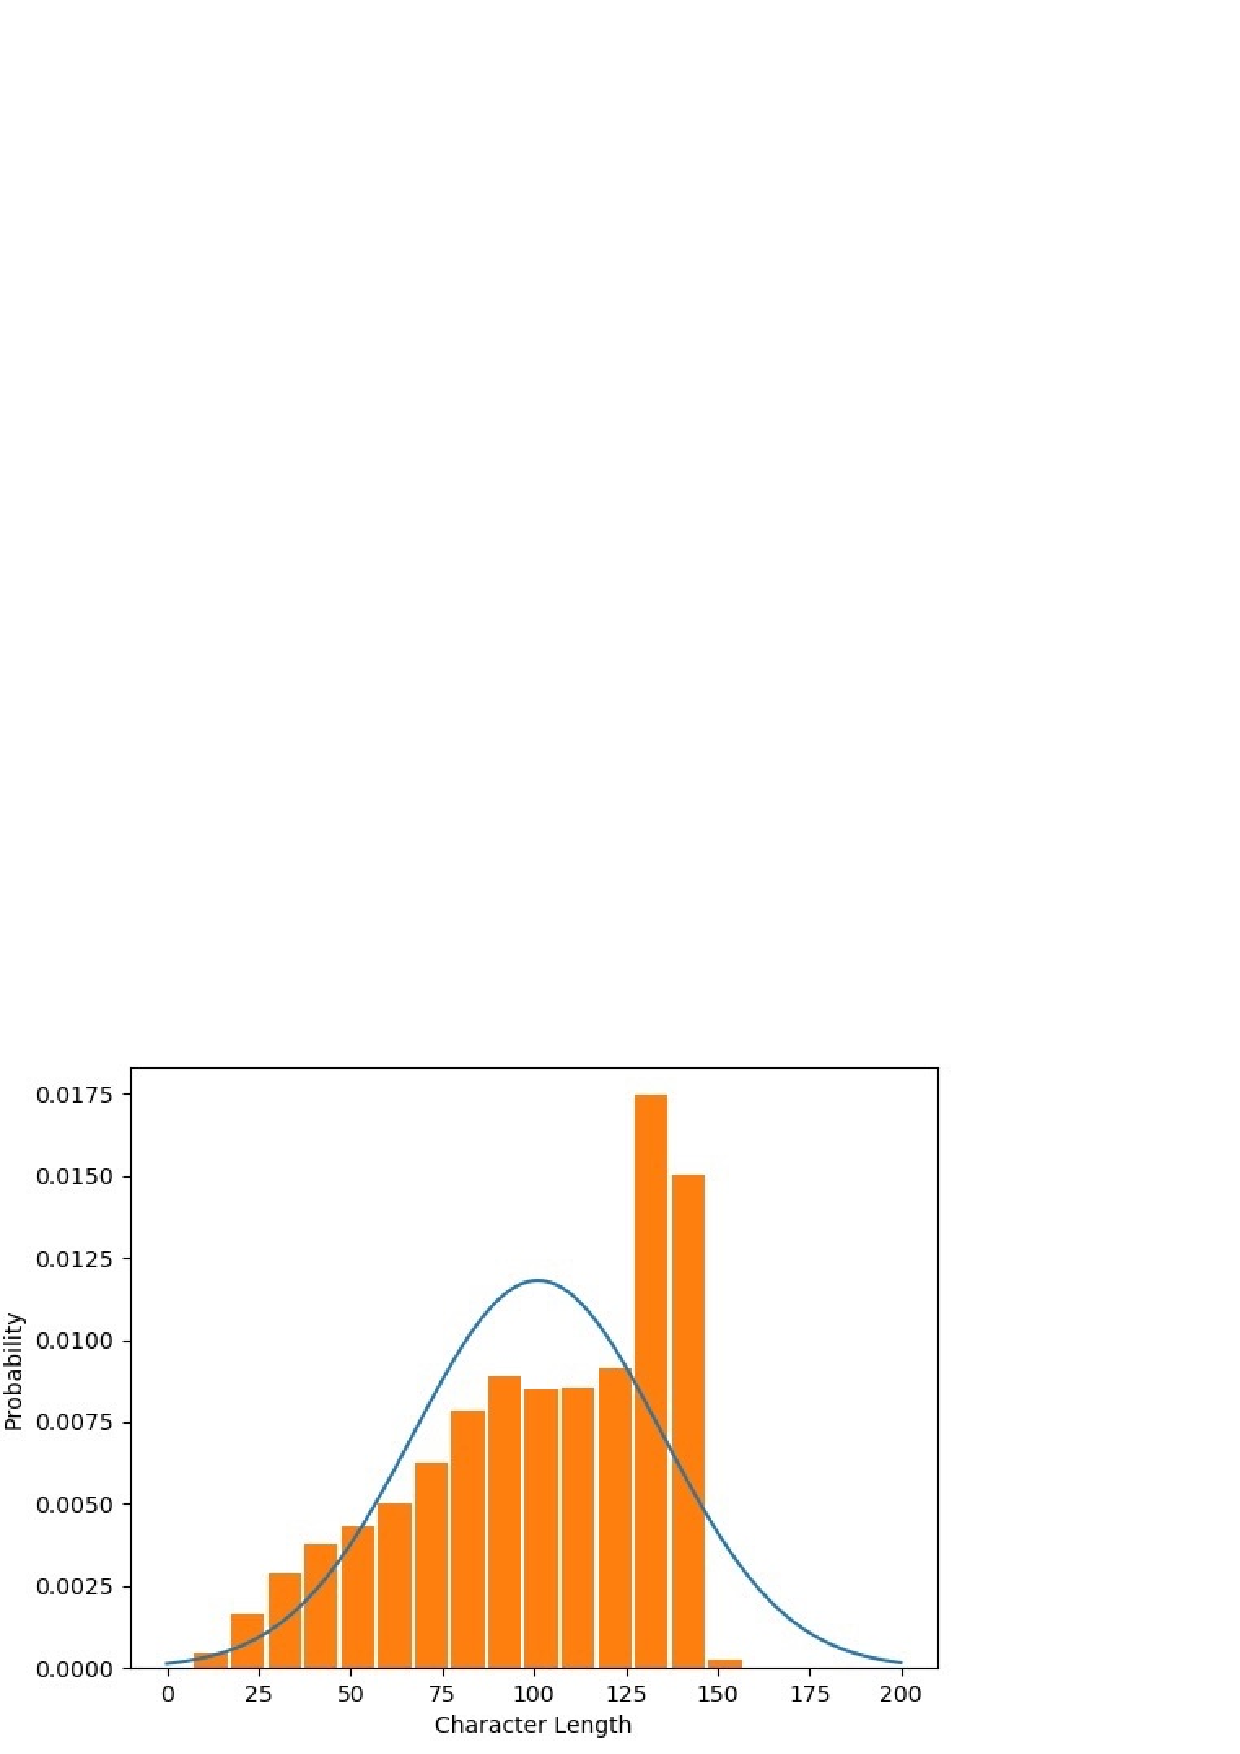
\includegraphics[width=1.0\linewidth]{figures//character dist.pdf}
      \end{tikzfigure}%
  \end{minipage}
  \hfill
  \begin{minipage}{0.5\linewidth}
      \centering
      \begin{tikzfigure}
        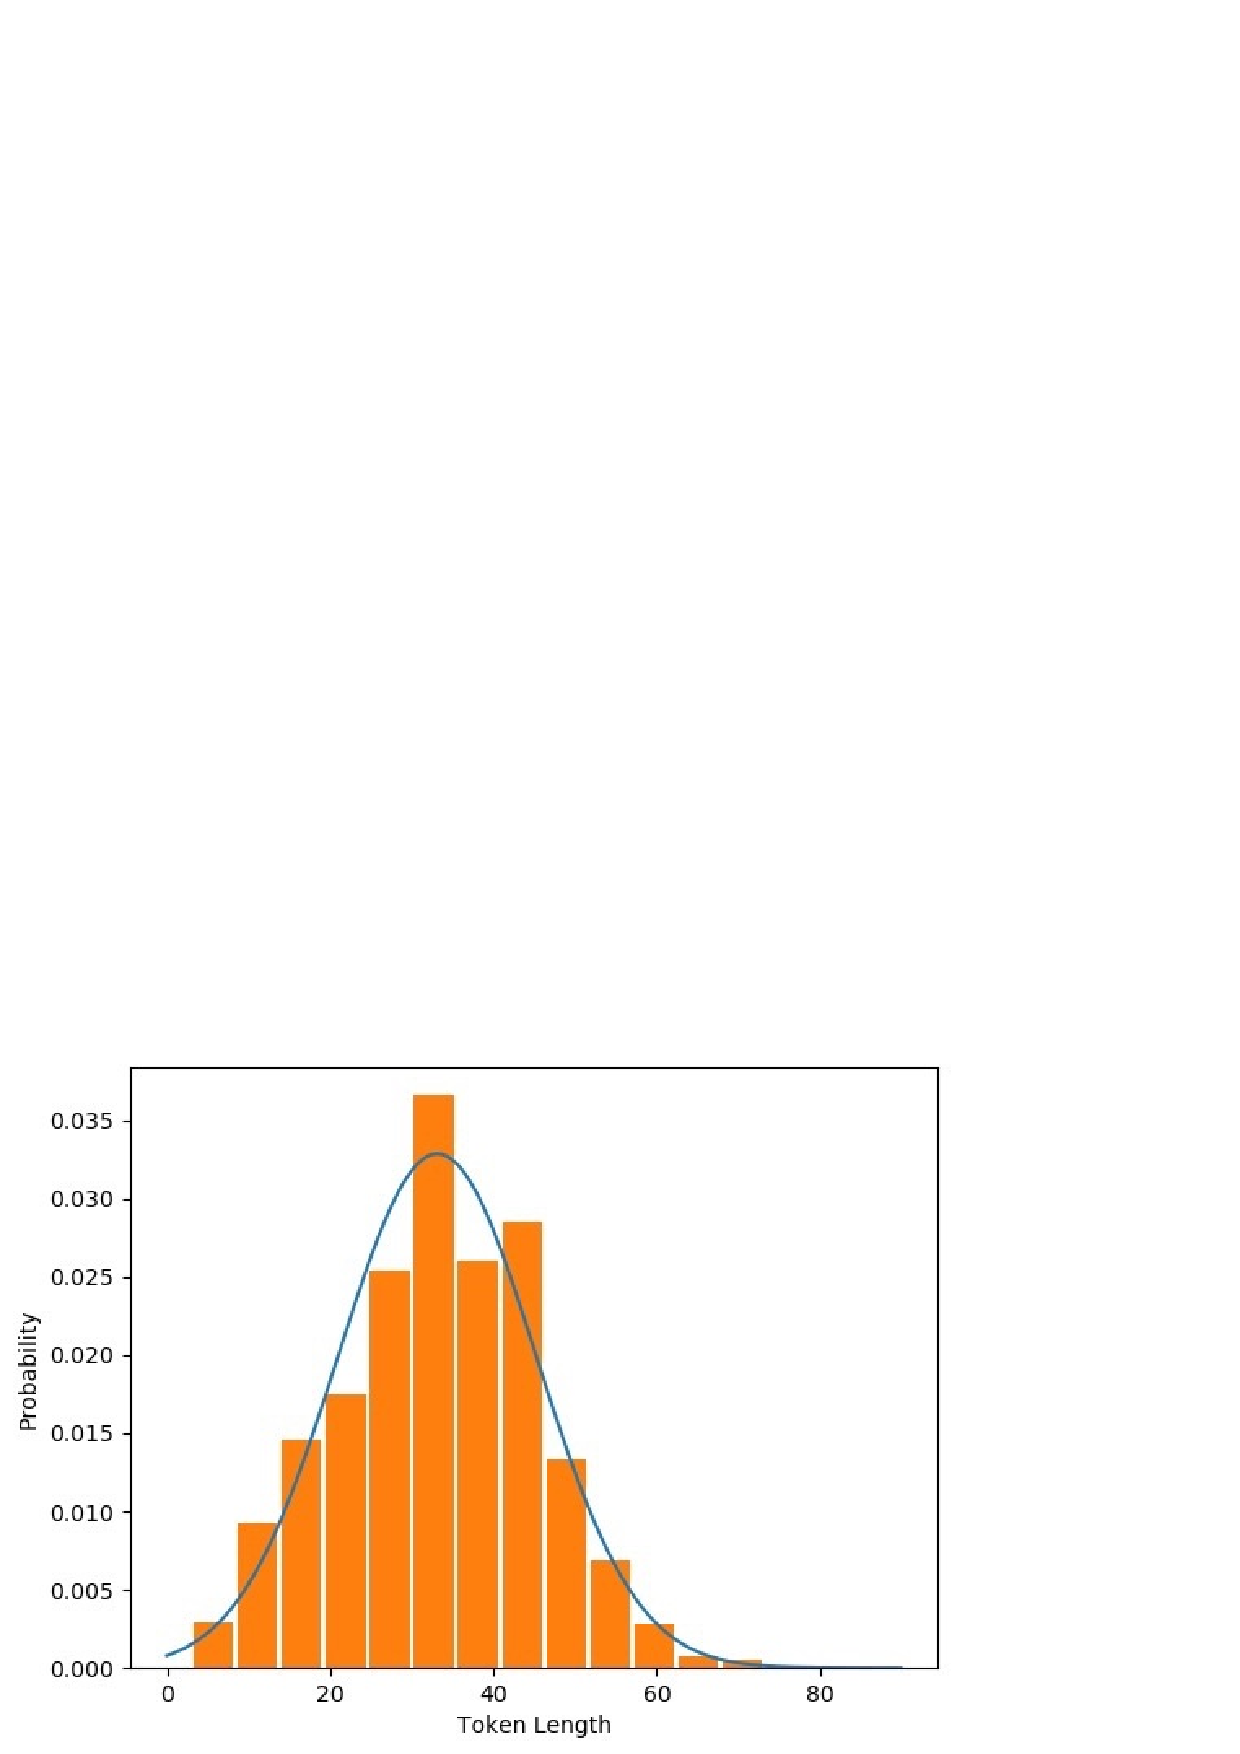
\includegraphics[width=1.0\linewidth]{figures//token dist.pdf}
      \end{tikzfigure}%
  \end{minipage}
  \vspace{.2cm}
  
  %  \begin{tikzfigure}
  %     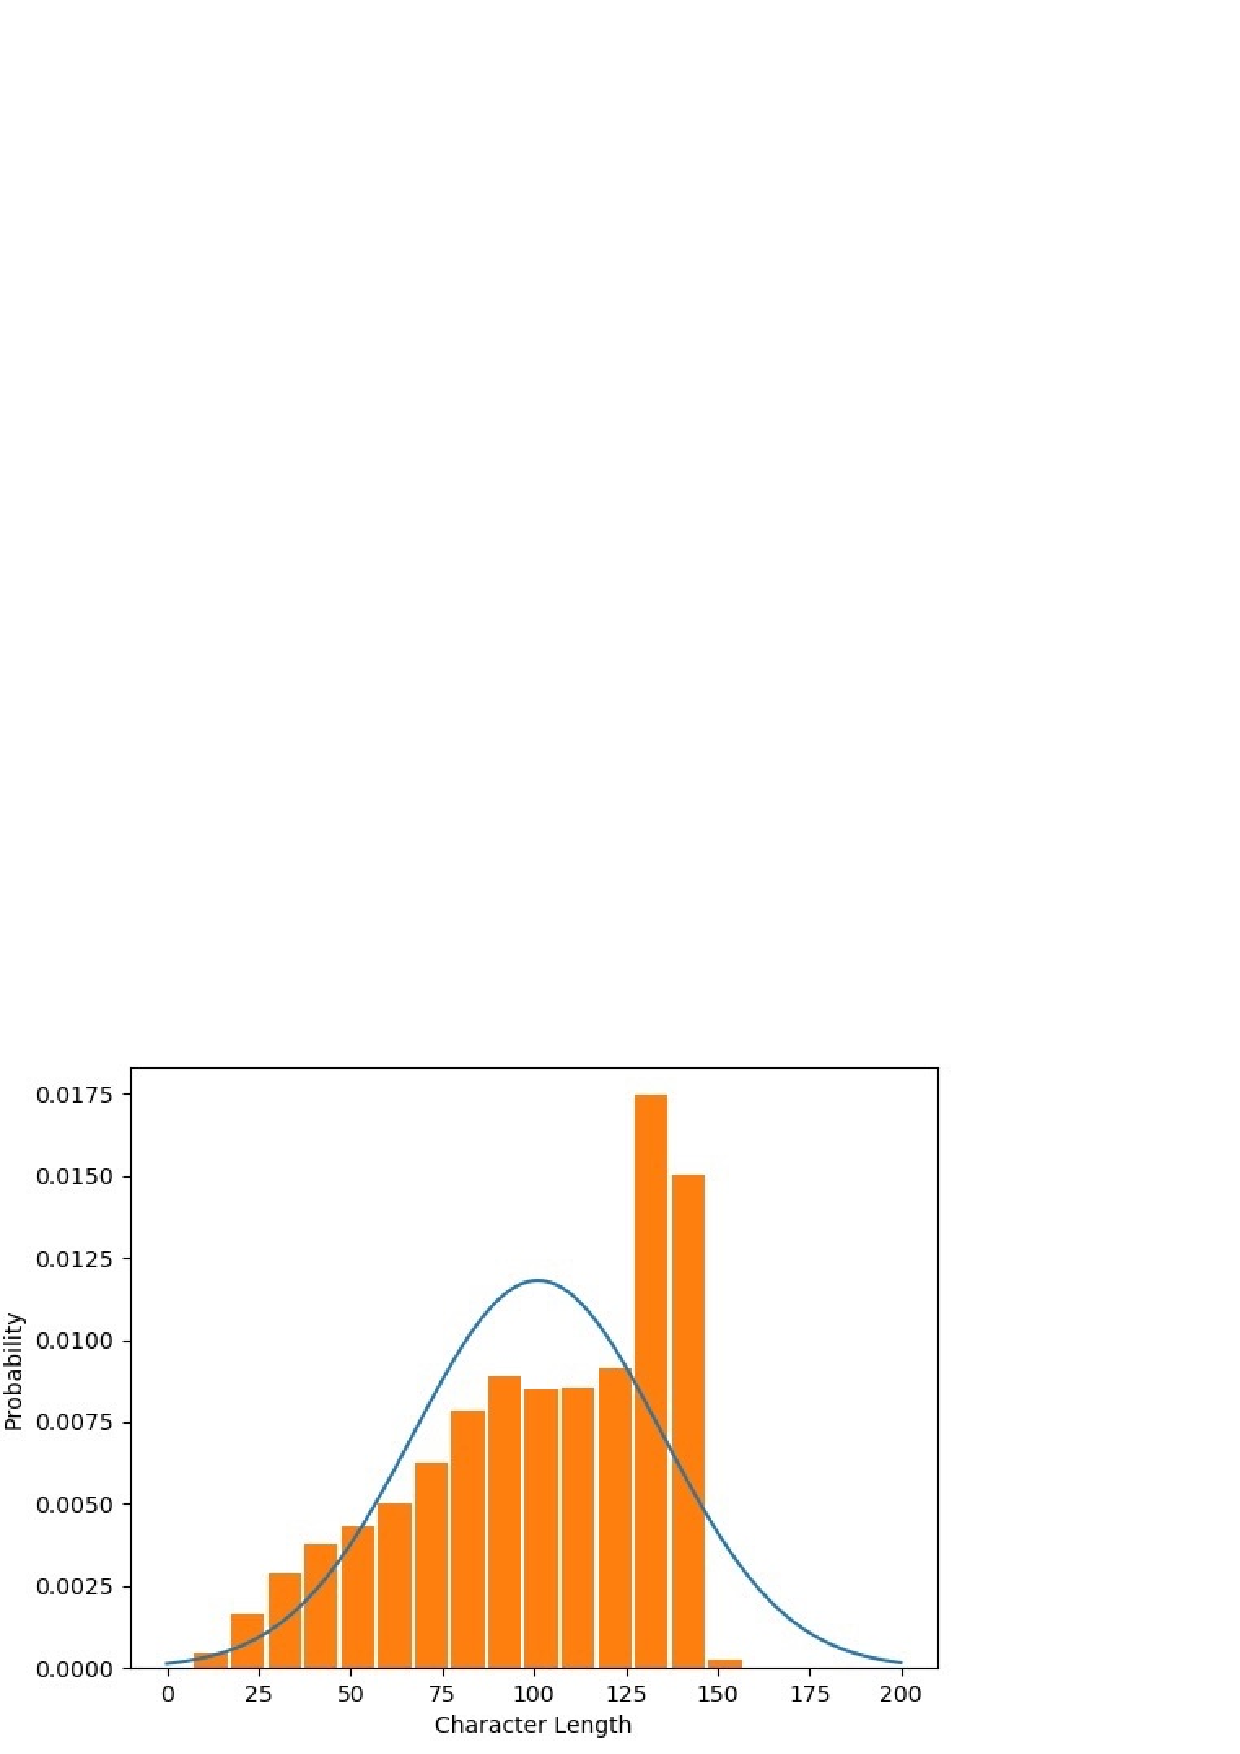
\includegraphics[width=0.8\linewidth]{figures//character dist.pdf}
  % \end{tikzfigure}

}
%%%%%%%%%% -------------------------------------------------------------------- %%%%%%%%%%


% SECOND column
\column{0.5}
 %Second column with first block's top edge aligned with with previous column's top.

%%%%%%%%%% -------------------------------------------------------------------- %%%%%%%%%%
\block{Methodology}{
  \begin{itemize}
    \item
    \textbf{Input format:} In order to convert texts into vectors that BERT can process, we should transform each tweet text into three vector, which are token vector, mask vector, segment vector, respectively.
    \begin{itemize}
      \item \textbf{Token vector} represents index of each token according to the vocabulary, the rest is padded with 0.
      \item \textbf{Mask vector} is used to calculate attention score without considering the meaningless part which is padded with 0.
      \item \textbf{Segment vector} is used to split two sentences. For the case there is only one sentence, segment vector is a zero vector.
    \end{itemize}
    \bigskip
    \item
    \textbf{Model details}\\
    We use bert-base and bert-large as our classification model, each of which has cased and uncased versions. Furthermore, we compare with bert that uses whole word mask to verify the effectiveness of this method. Model details are as follows.
\end{itemize}

\vspace{.5cm}
\centering
\begin{tabular}{ l  c  c  c  c }
    \toprule
    Model    & Layer  & Hidden  & Attention & Mask      \\
    \midrule
    bert-base-cased   & 12    & 768    & 12   & Token  \\
    bert-base-uncased   & 12    & 768    & 12   & Token \\
    bert-large-cased    & 24     & 1024    & 16  & Token \\
    bert-large-uncased   & 24    & 1024   & 16    & Token \\
    bert-large-wwm-cased  & 24    & 1024    & 16   & Span  \\
    bert-large-wwm-uncased & 24    & 1024    & 16    & Span \\
     \bottomrule
\end{tabular}
\vspace{1cm}

\begin{itemize}
  \item
    \textbf{Training setup}
\end{itemize}

\vspace{.5cm}
\centering
\begin{tabular}{ l  c }
    \toprule
    Name  & Value \\
    \midrule
    Token length   & 256     \\
		Dropout rate     & 0.1    \\
    Train\ :\ Validation         & 8\ :\ 2   \\
    Batch size         & 16   \\
		Number of epochs         & 3   \\
		Optimizer         & Adam      \\
		$\beta_1$          & 0.9    \\
		$\beta_2$         & 0.999   \\
    Learning rate   & 5e-5, 3e-5, 2e-5   \\
     \bottomrule
\end{tabular}
}
%%%%%%%%%% -------------------------------------------------------------------- %%%%%%%%%%
% Second column - first block


%%%%%%%%%% -------------------------------------------------------------------- %%%%%%%%%%
\block[titleleft]{Results}
{
  \begin{itemize}
    \item
    \textbf{Evaluation metric}
  \end{itemize} 
  \centering
  ${F_1\ score}  = \frac{2\ *\ precision\ *\ recall}{precision\ +\ recall}$
  \bigskip \bigskip
  \begin{itemize}
    \item
    \textbf{Results}
  \end{itemize} 

  \vspace{.5cm}

\centering
\begin{tabular}{ l  c }
    \toprule
    Model   & ${F_1\ score}$ \\
    \midrule
    bert-base-cased   & 0.825    \\
		bert-base-uncased     & 0.831       \\
		bert-large-cased         & 0.830     \\
		\bf{bert-large-uncased}   & \bf{0.848}      \\
		bert-large-wwm-cased         & 0.828    \\
		bert-large-wwm-uncased        & 0.825      \\
     \bottomrule
\end{tabular}

\vspace{1cm}
\begin{itemize}
  \item
  \textbf{Rank: }21/887\ \ $( 2.3$\%$)$
\end{itemize} 

}
%%%%%%%%%% -------------------------------------------------------------------- %%%%%%%%%%


% Second column - second block
%%%%%%%%%% -------------------------------------------------------------------- %%%%%%%%%%
\block[titleleft]{Limitation}
{
\begin{description}
Limited by computing resources, models are not fully trained, and no other pre-trained language models are used to compare with BERT.
\end{description}
}
%%%%%%%%%% -------------------------------------------------------------------- %%%%%%%%%%


% Bottomblock
%%%%%%%%%% -------------------------------------------------------------------- %%%%%%%%%%


%\note[targetoffsetx=8cm, targetoffsety=-10cm,rotate=0,angle=180,radius=8cm,width=.46\textwidth,innersep=.1cm]{
%Acknowledgement
%}

%\block[titlewidthscale=0.9, bodywidthscale=0.9]
%{Acknowledgement}{
%}
%%%%%%%%%% -------------------------------------------------------------------- %%%%%%%%%%

\end{columns}


%%%%%%%%%% -------------------------------------------------------------------- %%%%%%%%%%
%[titleleft, titleoffsetx=2em, titleoffsety=1em, bodyoffsetx=2em,%
%roundedcorners=10, linewidth=0mm, titlewidthscale=0.7,%
%bodywidthscale=0.9, titlecenter]

%\colorlet{noteframecolor}{blue!20}
\colorlet{notebgcolor}{blue!20}
\colorlet{notefrcolor}{blue!20}
\note[targetoffsetx=-13cm, targetoffsety=-6cm,rotate=0,angle=180,radius=8cm,width=.96\textwidth,innersep=.4cm]
{
\begin{minipage}{0.3\linewidth}
\centering
\includegraphics[width=24cm]{./graphics/logos/tulip-wordmark.eps}
\end{minipage}
\begin{minipage}{0.7\linewidth}
{ \centering
Disaster Tweets Prediction Using BERT,\ 14/11/2022,\ Beijing,\ China
}
\end{minipage}
}
%%%%%%%%%% -------------------------------------------------------------------- %%%%%%%%%%


\end{document}

%\endinput
%%
%% End of file `tikzposter-template.tex'.
